%% 519 drivers/scsi                   67% with stableCC
%% 531 fs                             69%
%% 572 arch/arm                       62%
%% 750 mm                             64%
%% 804 include                        53%
%% 973 arch/x86                       63%
%% 1083 kernel                         65%
%% 1323 sound                          83%
%% 1730 drivers/usb                    84%
%% 2126 drivers/gpu                    81%
%% 2418 drivers/net                    36%
%% 2887 net                            18%

%% 519 drivers/scsi                   8% in stable
%% 531 fs                             13%
%% 572 arch/arm                       4%
%% 750 mm                             13%
%% 804 include                        4%
%% 973 arch/x86                       10%
%% 1083 kernel                         11%
%% 1323 sound                          9%
%% 1730 drivers/usb                    17%
%% 2126 drivers/gpu                    7%
%% 2418 drivers/net                    6%
%% 2887 net                            11%


\documentclass{article}
\usepackage{pgfplots}
\pgfplotsset{width=3in,height=1.5in,compat=1.15}
\begin{document}
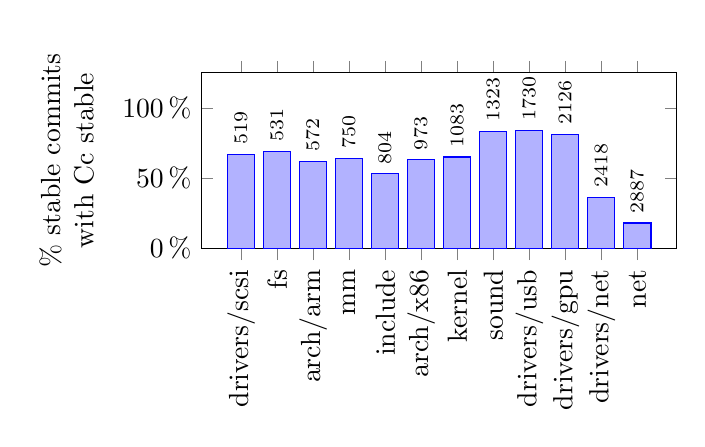
\begin{tikzpicture}
\usetikzlibrary{calc}
\begin{axis}[ybar,xtick=data,
 x tick label style={rotate=90,anchor=east, yshift=-0.01em},
ylabel={\begin{tabular}{c}\% stable commits\\with Cc stable\end{tabular}},
yticklabel=\pgfmathprintnumber{\tick}\,$\%$,
        ymin=0,
        ymax=125,
symbolic x
    coords={drivers/scsi,fs,arch/arm,mm,include,arch/x86,kernel,sound,drivers/usb,drivers/gpu,drivers/net,net}]
\addplot coordinates
{(drivers/scsi,                   67)
(fs,                             69)
(arch/arm,                       62)
(mm,                             64)
(include,                        53)
(arch/x86,                       63)
(kernel,                         65)
(sound,                          83)
(drivers/usb,                    84)
(drivers/gpu,                    81)
(drivers/net,                    36)
(net,                            18)};

\node[below,rotate=90,anchor=west] at (axis cs:drivers/scsi,67) {\scriptsize 519};
\node[below,rotate=90,anchor=west] at (axis cs:fs,69) {\scriptsize 531};
\node[below,rotate=90,anchor=west] at (axis cs:arch/arm,62) {\scriptsize 572};
\node[below,rotate=90,anchor=west] at (axis cs:mm,64) {\scriptsize 750};
\node[below,rotate=90,anchor=west] at (axis cs:include,53) {\scriptsize 804};
\node[below,rotate=90,anchor=west] at (axis cs:arch/x86,63) {\scriptsize 973};
\node[below,rotate=90,anchor=west] at (axis cs:kernel,65) {\scriptsize 1083};
\node[below,rotate=90,anchor=west] at (axis cs:sound,83) {\scriptsize 1323};
\node[below,rotate=90,anchor=west] at (axis cs:drivers/usb,84) {\scriptsize 1730};
\node[below,rotate=90,anchor=west] at (axis cs:drivers/gpu,81) {\scriptsize 2126};
\node[below,rotate=90,anchor=west] at (axis cs:drivers/net,36) {\scriptsize 2418};
\node[below,rotate=90,anchor=west] at (axis cs:net,18) {\scriptsize 2887};

\end{axis}
\end{tikzpicture}



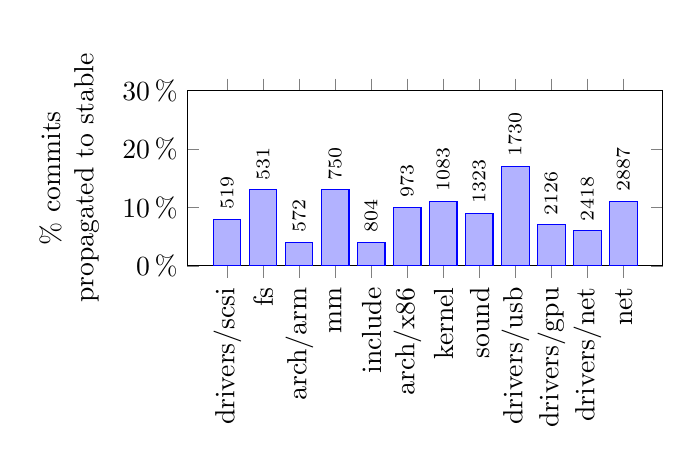
\begin{tikzpicture}
\usetikzlibrary{calc}
\begin{axis}[ybar,xtick=data,
 x tick label style={rotate=90,anchor=east, yshift=-0.01em},
ylabel={\begin{tabular}{c}\% commits\\propagated to stable\end{tabular}},
yticklabel=\pgfmathprintnumber{\tick}\,$\%$,
        ymin=0,
        ymax=30,
symbolic x
    coords={drivers/scsi,fs,arch/arm,mm,include,arch/x86,kernel,sound,drivers/usb,drivers/gpu,drivers/net,net}]
\addplot coordinates
{(drivers/scsi,                   8)
(fs,                             13)
(arch/arm,                       4)
(mm,                             13)
(include,                        4)
(arch/x86,                       10)
(kernel,                         11)
(sound,                          9)
(drivers/usb,                    17)
(drivers/gpu,                    7)
(drivers/net,                    6)
(net,                            11)};

\node[below,rotate=90,anchor=west] at (axis cs:drivers/scsi,8) {\scriptsize 519};
\node[below,rotate=90,anchor=west] at (axis cs:fs,13) {\scriptsize 531};
\node[below,rotate=90,anchor=west] at (axis cs:arch/arm,4) {\scriptsize 572};
\node[below,rotate=90,anchor=west] at (axis cs:mm,13) {\scriptsize 750};
\node[below,rotate=90,anchor=west] at (axis cs:include,4) {\scriptsize 804};
\node[below,rotate=90,anchor=west] at (axis cs:arch/x86,10) {\scriptsize 973};
\node[below,rotate=90,anchor=west] at (axis cs:kernel,11) {\scriptsize 1083};
\node[below,rotate=90,anchor=west] at (axis cs:sound,9) {\scriptsize 1323};
\node[below,rotate=90,anchor=west] at (axis cs:drivers/usb,17) {\scriptsize 1730};
\node[below,rotate=90,anchor=west] at (axis cs:drivers/gpu,7) {\scriptsize 2126};
\node[below,rotate=90,anchor=west] at (axis cs:drivers/net,6) {\scriptsize 2418};
\node[below,rotate=90,anchor=west] at (axis cs:net,11) {\scriptsize 2887};

\end{axis}
\end{tikzpicture}
\end{document}
